\section {Assignment 3 \\ {Moving Object}}
\label {sec:assignment_3}

Take an image of a considerably fast moving object (rotating disk) without any motion-blur and without reflection from any light-sources. You will not be able to synchronize the camera, so find a solution which will not need any synchronization.
Make a sketch of the required setup first, discuss multiple solutions in the group. \cite{Lab_Assignments}



\begin{lstlisting}[language=C, caption=save image to file, label=lst:50loop]
// capture 50 frames
if (capt50 == true) {
    capt50 = false;
    for(int i = 0; i < 50; i++) {
        cam0.captureFrame(&image);
        // save image with frame number
        imwrite("../capt/img" + to_string(i) + ".png", image);
    }
}
\end{lstlisting}


\subsection{Optimal exposure}

We use a strobe light to expose this image. The stroke frequency is not important but should be sufficiently slow to make it impossible for two exposures to occur in a single frame, and it should also be slow so that the capacitors inside the strobe enough time to charge to give the lights its maximum brightness. We took 50 images, and saved them to the file system. The first image which looks like \ref{fig:img36} was handpicked and the other images ware ignored.

\begin{figure}[h!]
    \centering
    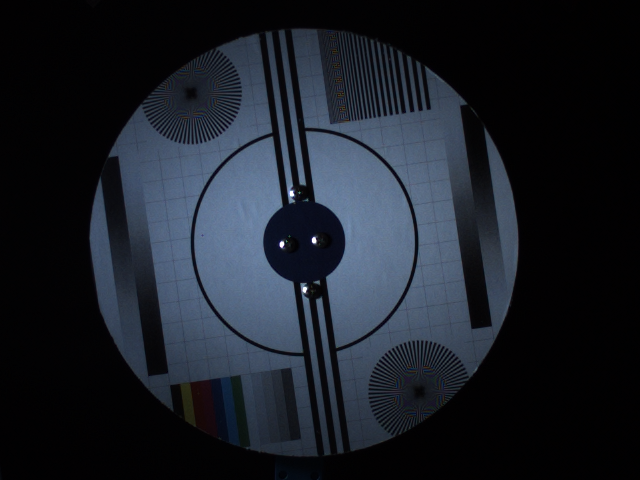
\includegraphics[width=0.35\textwidth]{img36.png}
    \caption{Image of moving object}
    \label{fig:img36}
\end{figure}

\subsection{Sketch of setup}

\begin{figure}[h!]
    \centering
    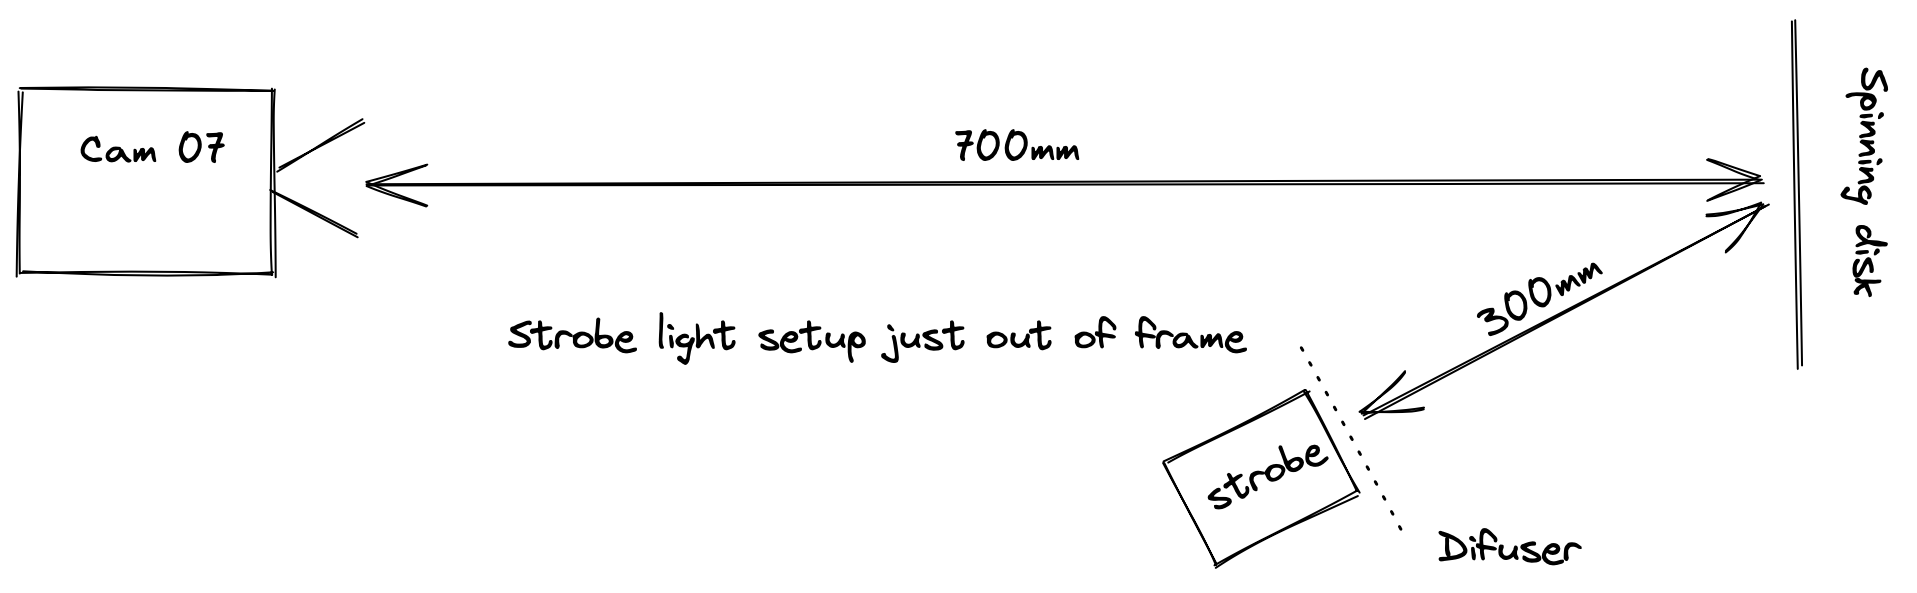
\includegraphics[width=0.65\textwidth]{Lab_3_Diagram.png}
    \caption{Sketch of setup}
    \label{fig:Lab_3_Diagram}
\end{figure}

\subsection{Calculation of ‘angle of view’}

We use the same camera and lens as assignment two, So the angle of view will be identical as calculated in section \ref{sec:angle_of_view}.